\documentclass{article}
\usepackage{amsmath}
\usepackage{subcaption}
\usepackage{graphicx}
\begin{document}
    \section{}
    '''
    This formula $f(x) = x^2$ is an example.\\
    '''
    $z = \frac{x}{y}$\quad $C_1 \quad = \quad c_2 + c_4^3$\\
    \begin{equation*}
        1 + 2 = 3\\
        f(x) = x_1 + x_2^2 + x_3^3
    \end{equation*}
    \begin{equation*}
        1 = 3 - 2
    \end{equation*}
    \begin{equation*}
        1 * 8 = 8
    \end{equation*}
    \begin{align*}
        1 + 2 &= 3\\
        1 &= 3-2
    \end{align*}

    \begin{align*}
        f(x) &= x^2\\
        g(x) &= \frac{1}{3}x^3\\
        F(x) &= \int^a_b \frac{1}[3]x^3\\
        t(x) &= \frac{1}{\sqrt{x}}\\
    \end{align*}
    $\begin{matrix}
        1 & 0\\
        0 & 1\\
        3 & 4
    \end{matrix}\\
    \left[
        \begin{matrix}
            1 & 10\\
            10 & 1
        \end{matrix}
    \right]\\
    \left(\frac{1}{\sqrt{x}}\right)
    $
    $[
        \begin{matrix}
            1 & 0\\
            0 & 1
        \end{matrix}
    ]$
    \begin{figure}
        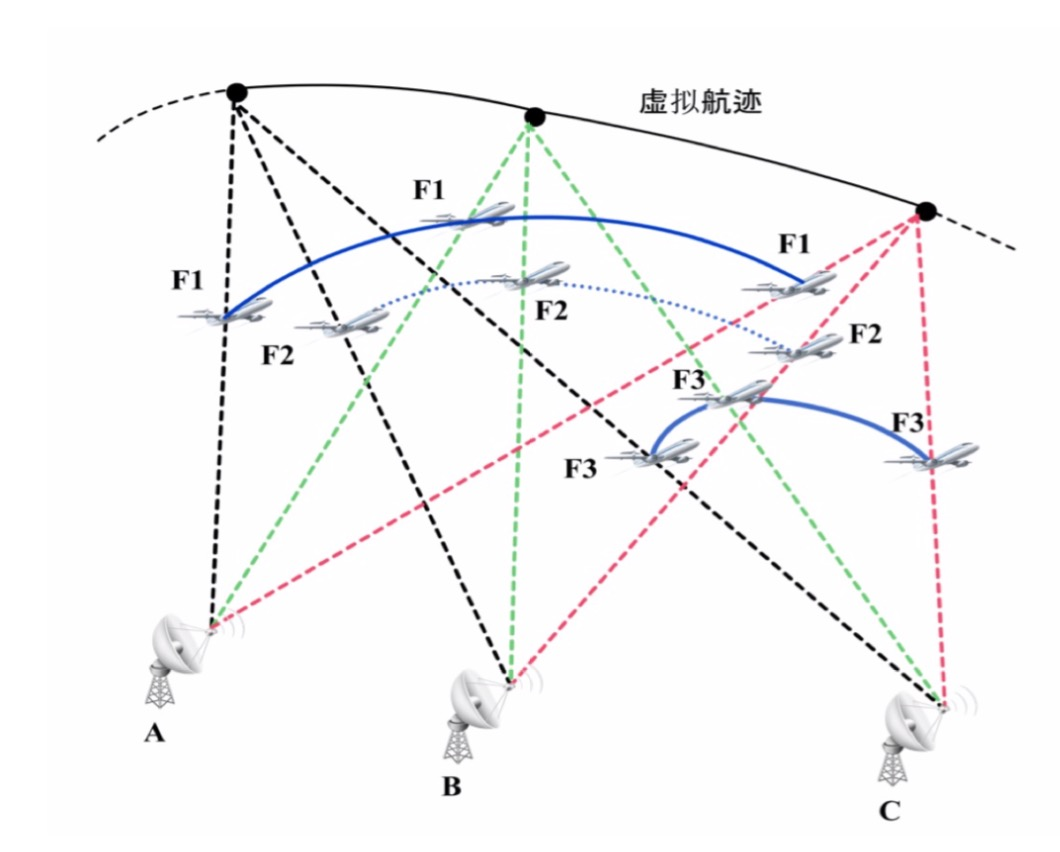
\includegraphics[width=\linewidth]{LatexTeample/test.jpg}
        \caption{A piture.}
        \label{fig:p1}
    \end{figure}
    % Figure \ref{fig:p1} show a boat.
    %...
    
    \begin{figure}[h!]
        \centering
        \begin{subfigure}[b]{0.4\linewidth}
            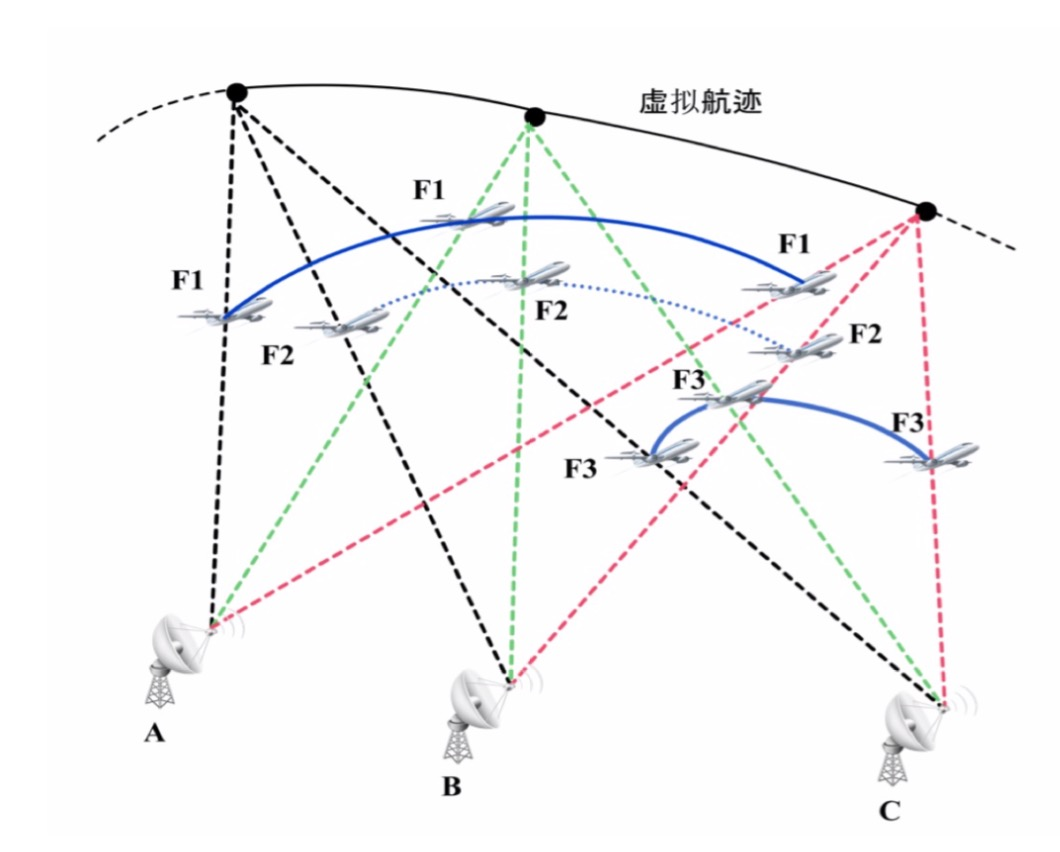
\includegraphics[width=\linewidth]{LatexTeample/test.jpg}
            \caption{virtual trace.}
        \end{subfigure}
        \begin{subfigure}[b]{0.5\linewidth}
            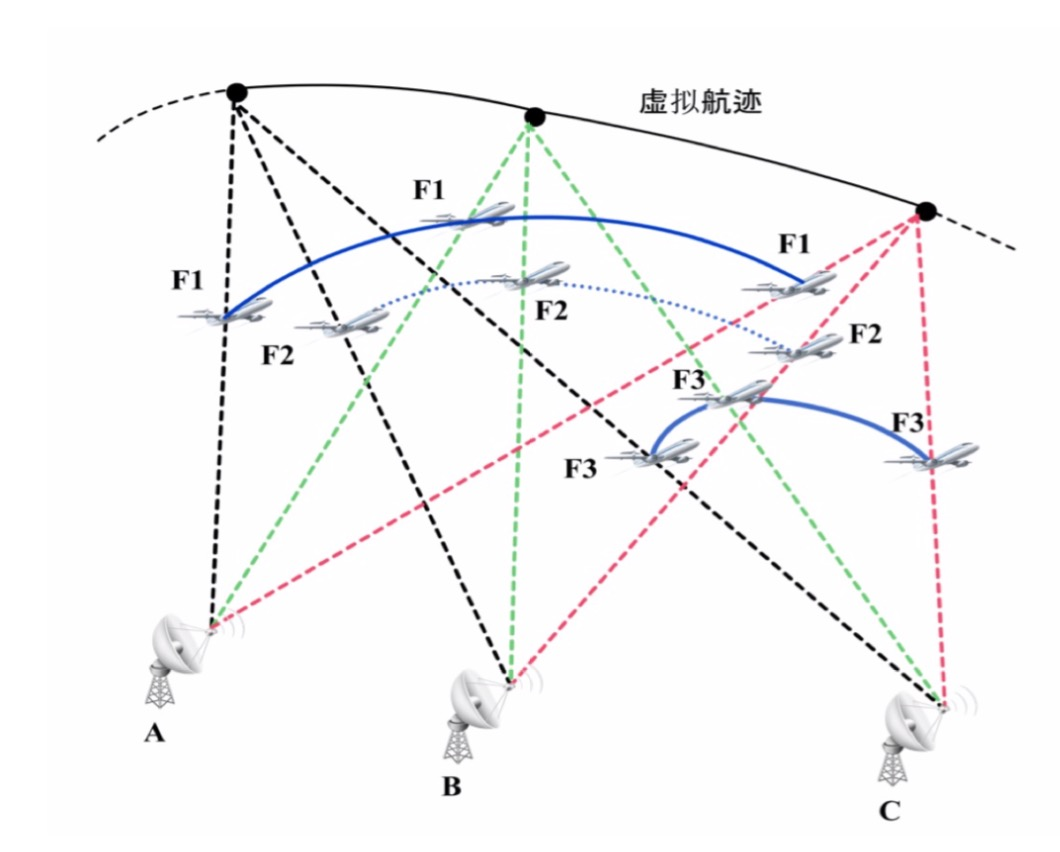
\includegraphics[width=\linewidth]{LatexTeample/test.jpg}
            \caption{more virtual trace.}
        \end{subfigure}
        \caption{The same photo of trace.}
        \label{fig:trace}
    \end{figure}

    %...
    % table content
    \tableofcontents
    \newpage
    \section{Section}
    dummy text
    \subsection{Subsection}
    dummy text1
    \begin{table}
        \caption{Dummy table}
    \end{table}
    \begin{appendix}
        \listoffigures
        \listoftables
\end{document}